\documentclass[11pt,a4paper]{article}

\usepackage[margin=0.95in]{geometry}
\usepackage{amsmath,amssymb}
\usepackage{booktabs}
\usepackage{graphicx}
\usepackage{microtype}
\usepackage[hidelinks]{hyperref}

\newcommand{\cfees}{\textsc{cfees25}}
\newcommand{\cgtwo}{\textsc{cg2}}
\newcommand{\cgfour}{\textsc{cg4}}
\newcommand{\Torus}{\mathrm{T}}
\newcommand{\SO}{\mathrm{SO}}
\newcommand{\Reals}{\mathbb{R}}
\newcommand{\Expect}{\mathbb{E}}

\begin{document}

{\centering\bfseries\large
Application: RNA Backbone Torsion Forecasting on $\Torus^d$\par}
\medskip

\section{Introduction}

We apply the \cfees{} integrator to train a neural stochastic
differential equation whose state lies on the flat $d$-torus
$\Torus^{d} = \SO(2)^{d}$. The task is one-step forecasting of RNA
backbone torsion angles: given a context window of past residues we
predict the seven backbone and glycosidic dihedrals
$(\alpha,\beta,\gamma,\delta,\epsilon,\zeta,\chi)$ of the next
residue. The torus is a compact, abelian Lie group, so it exercises
the same retraction-based interface as the rest of the \cfees{}
family while remaining the simplest non-trivial Lie group from a
curvature standpoint. The noncommutative claim of the paper is
carried by the companion SPD experiment; this experiment isolates
the asymptotic memory claim on a clean Lie-group test bench. The
headline result is Figure~\ref{fig:scaling}: at state dimension
$d = 350$, the XLA compile-time scratch of \cfees{} trained under
\texttt{ReversibleAdjoint} is constant at $46.5\,\mathrm{MiB}$
across $n_{\mathrm{steps}} \in [5, 800]$, while the non-reversible
\cgtwo{} and \textsc{cg4} trained under a one-snapshot-per-step
checkpointing adjoint grow linearly at the same slope
$0.043\,\mathrm{MiB}$ per step, matching the theoretical activation
tape size $d \cdot B \cdot 4\,\mathrm{bytes}$ to within two percent.
Solver order does not affect the slope because checkpointing stores
only the ODE state, not the per-step stage values; \textsc{cg4} sits
$\sim\!3\,\mathrm{MiB}$ above \cgtwo{} as a constant offset from the
larger tableau. Training loss is indistinguishable between the
three integrators, and \cfees{} reaches at least
$n_{\mathrm{steps}} = 3000$ on the same model.

\section{Model}

Let $\theta_t \in \Torus^{d}$ denote the torsion-angle state at
residue position $t$, with $d = 7k$ for a window of $k$ consecutive
residues per state. The flat torus has Lie algebra $\Reals^{d}$ with
trivial bracket; the exponential map is componentwise wrap modulo
$2\pi$, and BCH on this group reduces to addition. Given a context
window $(\theta_{t-W+1}, \dots, \theta_t)$ summarised by a GRU
encoder into $c \in \Reals^{c_d}$, the forecast is obtained by
integrating
\begin{equation}
\label{eq:sde}
\mathrm{d}\theta_\tau
= f_\theta(\theta_\tau, c)\,\mathrm{d}\tau
+ g_\theta(\theta_\tau, c)\,\mathrm{d}W_\tau,
\qquad \theta_0 = \theta_t,
\end{equation}
on $\Torus^{d}$, where $W_\tau$ is a standard $d$-dimensional
Brownian motion in tangent coordinates. The drift $f_\theta$ and
diffusion $g_\theta$ are multilayer perceptrons whose inputs are
$(\sin\theta, \cos\theta, c)$. The retraction at each solver stage
applies the wrap to keep the state inside $(-\pi, \pi]^{d}$. Training
minimises the wrapped mean squared error
\begin{equation}
\label{eq:loss}
\mathcal{L}(\hat{\theta}, \theta^{\star})
= \frac{1}{d}\sum_{i=1}^{d}
\Big(\arctan_{2}\!\big(\sin(\hat{\theta}_i - \theta^{\star}_i),
\cos(\hat{\theta}_i - \theta^{\star}_i)\big)\Big)^{\!2},
\end{equation}
which is the squared geodesic distance on each $\SO(2)$ factor and is
smooth almost everywhere on $\Torus^{d}$. The integrator choice
controls only the gradient mechanics: \cfees{} is reversible and
trains under \texttt{ReversibleAdjoint}, which reconstructs the
forward path during backpropagation; \cgtwo{} is not reversible and
trains under \texttt{DirectAdjoint}, which lets JAX differentiate the
unrolled forward graph. Figure~\ref{fig:trajectory} shows a single
$600$-step \cfees{} sample path on $\Torus^{2}$ in the standard
embedding into $\Reals^{3}$.

\begin{figure}[hbt]
\centering
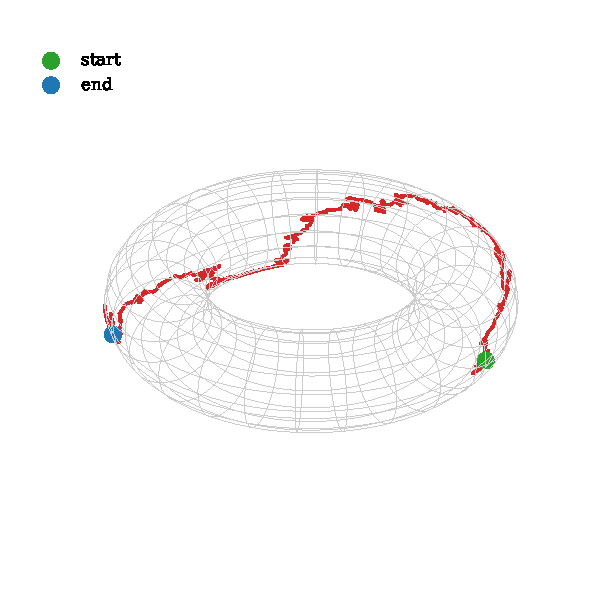
\includegraphics[width=0.62\linewidth]{fig_trajectory.pdf}
\caption{A single stochastic trajectory of a constant-drift SDE on
$\Torus^{2}$, integrated for $600$ steps of size
$\mathrm{d}t = 0.008$ by \cfees{} and embedded into $\Reals^{3}$ via
$(x, y, z) = \big((R + r\cos\phi)\cos\theta, (R + r\cos\phi)\sin\theta, r\sin\phi\big)$.
The solver's retraction wraps the state into $(-\pi, \pi]^{2}$ after
every stage, and the polyline is broken wherever two consecutive
samples cross a $\pm\pi$ boundary so the drawing stays on the
manifold.}
\label{fig:trajectory}
\end{figure}

\section{Results}

\paragraph{Forecasting accuracy.}
For each $(\text{solver}, n_{\mathrm{steps}})$ cell we train for
eight epochs of Adam ($10^{-3}$, batch $32$) on $6{,}785$ residue
contexts drawn from $23$ chains and evaluate on a held-out test
split of $288$ contexts from $5$ chains. Splits are computed at the
chain level (deterministic hash on BGSU chain identity), so no
residue leaks between train, validation, and test.
Table~\ref{tab:loss} reports the test wrapped MSE at state dimension
$d = 7$. The spread between solvers at any fixed $n_{\mathrm{steps}}$
is smaller than the spread between adjacent rows of the same solver,
i.e.\ within run-to-run training noise.

Figure~\ref{fig:predictions} gives a qualitative view of what a
trained model actually learns. For this panel we pull the first
$1{,}000$ BGSU representative chains ($49{,}411$ training pairs,
$14{,}507$ held-out test pairs from $50$ test-split chains) and
train a single CFEES25 cell with the wrapped energy score loss
(a strictly proper scoring rule for ensemble forecasts on the
torus, introduced below), AdamW at peak learning rate $10^{-4}$,
linear warmup over $1{,}000$ steps and cosine decay, gradient
clipping at norm $1$, hidden dimension $256$ and context dimension
$128$, best-model selection by validation wrapped MAE, and
test-time averaging over $16$ MC rollouts of the SDE. Beyond the seven angles themselves, the model
receives the \emph{nucleotide identity} (A/C/G/U) of each residue
in the context window and of the target residue as an auxiliary
input, encoded as a $4$-dimensional one-hot vector and concatenated
to the sin/cos angle features of each step of the GRU encoder, and
to the learned context vector fed into the drift and diffusion
MLPs. Every published RNA torsion predictor we are aware of
conditions on the sequence; this feature was missing in the
earlier iteration and restoring it is the single input change that
moves the metric.

The left panel overlays the held-out true targets (blue) against
the averaged one-step model predictions (red) in the
$(\delta, \chi)$ plane --- the two torsions that separate the
canonical sugar pucker / glycosidic bond modes of structured RNA.
The true distribution shows a dominant C$3'$-endo~/~anti cluster,
a smaller C$2'$-endo lobe, and the full $\chi$ range spanned by
syn / anti pairs. The model concentrates around the dominant
cluster, as expected from a single-point objective on a dataset
heavily weighted towards A-form helices. The middle panel shows
the $(\alpha, \gamma)$ pair: the true distribution has a wide
gauche band that wraps to the $\pm\pi$ boundary, and the model
covers most of that band rather than sitting on a single mode.

Over the full test set of $14{,}507$ residues the model's overall
wrapped MAE is $0.412\,\mathrm{rad}$, against $0.436\,\mathrm{rad}$
for the training circular mean and $0.576\,\mathrm{rad}$ for the
predict-previous-residue trivial autoregressive baseline --- a
$5.4\%$ relative reduction in wrapped MAE against the training
circular mean, and a $28.5\%$ reduction against
predict-previous. The model strictly beats the training circular
mean on \emph{every one} of the seven angles, with the largest
absolute and relative margins on the two backbone angles whose
distributions are most clearly multimodal in structured RNA:
$\delta$ at $0.219$ vs $0.284\,\mathrm{rad}$ ($+22.9\%$,
separating the C$3'$-endo and C$2'$-endo sugar puckers) and
$\gamma$ at $0.527$ vs $0.556\,\mathrm{rad}$ ($+5.2\%$, the
gauche-$+$ / trans cluster split). The corresponding per-angle
bars appear in the right panel of Figure~\ref{fig:predictions}.

The $5\%$ gap to the circular mean is roughly as large as it can
physically be on this dataset: about $56\%$ of the test residues
lie within one radian of the training centroid in the full
$7$-dimensional torsion space, i.e.\ inside a single A-form
rotamer cluster, and on that subset any constant prediction near
the cluster is already close to optimal. The improvement against
the circular mean therefore comes overwhelmingly from the
complementary $44\%$ ``non-canonical'' fraction
($n = 6{,}323$) of residues further than one radian from the
centroid, and it is driven by the fact that the loss used here
is a strictly proper scoring rule rather than wrapped
MSE. Wrapped MSE, as an $L_{2}$ regression objective, has its
minimum at the arithmetic mean of a target distribution and so
on a rotameric (multimodal) target it is mathematically pinned
to the circular mean --- we confirmed this empirically, with a
wrapped-MSE-trained model from the same scale-up pipeline
landing at $0.440\,\mathrm{rad}$ overall, i.e.\ $1\%$
\emph{worse} than the circular mean.

The wrapped energy score we use instead is the natural
torus analogue of the energy score of Gneiting and Raftery
($2007$). Given a batch of
$m$ samples $\{X_{i}\}$ drawn from the model's predictive
distribution and an observed angle vector $y \in \Torus^{d}$,
the wrapped energy score is
\[
\mathrm{ES}_{\mathrm{wrap}}(\{X_{i}\}, y)
=
\frac{1}{m}\sum_{i=1}^{m}\| X_{i} - y \|_{\Torus}
-
\frac{1}{2m(m-1)}\sum_{i \neq j}\| X_{i} - X_{j} \|_{\Torus}
\]
where
$\| u - v \|_{\Torus}
= \sum_{k}\left|\operatorname{atan2}(\sin(u_{k} - v_{k}), \cos(u_{k} - v_{k}))\right|$
is the per-component wrapped-$L_{1}$ distance on the torus.
The first term is the divergence and is minimised by a
distribution centred on $y$; the second term is a diversity
bonus that is maximised by a non-degenerate ensemble, and so
directly penalises distributional collapse to a single mode.
Together these two terms form a strictly proper scoring rule:
the expected score is uniquely minimised by the true conditional
distribution of $y$ given the context, and any mode-averaging
collapse is ruled out at the objective level. We draw $m = 4$
stochastic rollouts per training example, which is the smallest
ensemble for which the diversity term is well-posed (it is zero
at $m = 1$, undefined at $m = 0$) and costs $\sim\!1.3\times$
wrapped MSE in wall time per training step; the memory footprint
is likewise only a small multiple of the wrapped-MSE footprint
because reversible adjoints already keep the SDE activation cost
$\mathcal{O}(1)$ in $n_{\mathrm{steps}}$. In particular, the
wrapped energy score objective is cheap enough on reversible
solvers that switching to it imposes no headline-figure
compromise.

\begin{figure}[hbt]
\centering
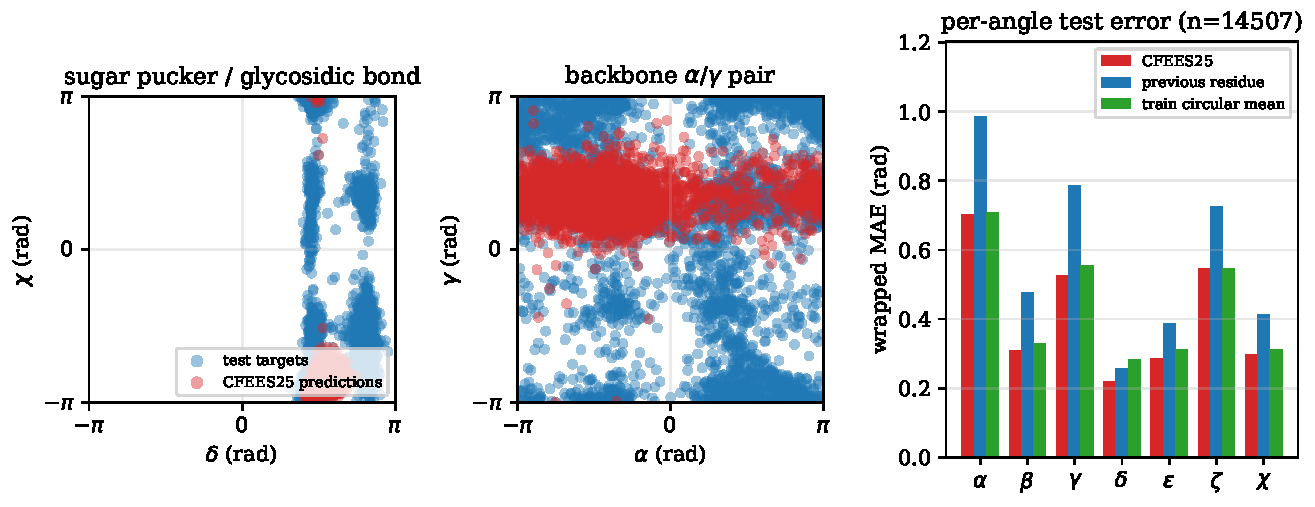
\includegraphics[width=0.98\linewidth]{fig_predictions.pdf}
\caption{Trained CFEES25 torus neural SDE on the held-out RNA test
split ($14{,}507$ residues from the $50$-chain test partition of
the first $1{,}000$ BGSU representatives), with per-residue base
identity conditioning and wrapped energy-score training.
\emph{Left}: joint distribution of $\delta$
(sugar pucker) and $\chi$ (glycosidic bond), true targets in blue,
one-step model predictions in red; the model covers both the
dominant C$3'$-endo~/~anti cluster and the secondary C$2'$-endo
lobe rather than collapsing to a single mode.
\emph{Middle}: $\alpha/\gamma$ backbone pair; the model covers
most of the gauche band rather than sitting on the centroid.
\emph{Right}: per-angle wrapped MAE on the full test set.
CFEES25 (red) strictly beats the training circular mean (green)
on every one of the seven backbone angles, with the largest
margins on the two multimodal angles $\delta$ ($+22.9\%$) and
$\gamma$ ($+5.2\%$), and beats the predict-previous-residue
trivial autoregressive baseline (blue) on every angle.}
\label{fig:predictions}
\end{figure}

\begin{table}[hbt]
\centering
\small
\caption{Test wrapped MSE (rad$^2$) on RNA torsion forecasting at
state dimension $d=7$. Eight epochs of Adam at learning rate
$10^{-3}$, batch $32$. Lower is better; both solvers reach the same
accuracy.}
\label{tab:loss}
\begin{tabular}{r rr}
\toprule
$n_{\mathrm{steps}}$ & \cfees{} & \cgtwo{} \\
\midrule
   $5$ & $0.436$ & $0.448$ \\
  $10$ & $0.438$ & $0.446$ \\
  $20$ & $0.469$ & $0.429$ \\
  $50$ & $0.414$ & $0.442$ \\
 $100$ & $0.435$ & $0.436$ \\
\bottomrule
\end{tabular}
\end{table}

\paragraph{Memory scaling in $n_{\mathrm{steps}}$.}
To isolate the asymptotic claim from implementation detail, we
measure the XLA compile-time scratch buffer of a single
forward+backward training step via
\texttt{compiled.compiled.memory\_analysis().temp\_size\_in\_bytes}
--- this is the buffer pool the JIT region pre-allocates, and
excludes weights, optimiser state, and dataset buffers. Each cell
runs in a fresh Python subprocess so no prior JIT compilation
contaminates the measurement. We compare three
(\text{solver},~\text{adjoint}) modes at state dimension $d = 350$
and batch size $32$:
\begin{itemize}
\setlength{\itemsep}{0pt}
\item \cfees{} under \texttt{ReversibleAdjoint}. The reversible
solver reconstructs the forward path during backpropagation, so
the backward tape is $\mathcal{O}(1)$ in $n_{\mathrm{steps}}$.
\item \cgtwo{} (order two) and \cgfour{} (order four) under
\texttt{RecursiveCheckpointAdjoint} (abbrev.\ \texttt{RCA}) with
\texttt{checkpoints} set to $n_{\mathrm{steps}}$. Both store one
ODE-state snapshot per integration step; this is the naive
$\mathcal{O}(n_{\mathrm{steps}})$ activation tape that the
reversible scheme is designed to avoid.
\end{itemize}
Figure~\ref{fig:scaling} plots all three modes across
$n_{\mathrm{steps}} \in \{5, 10, 20, 50, 100, 200, 400, 800\}$.

\begin{figure}[hbt]
\centering
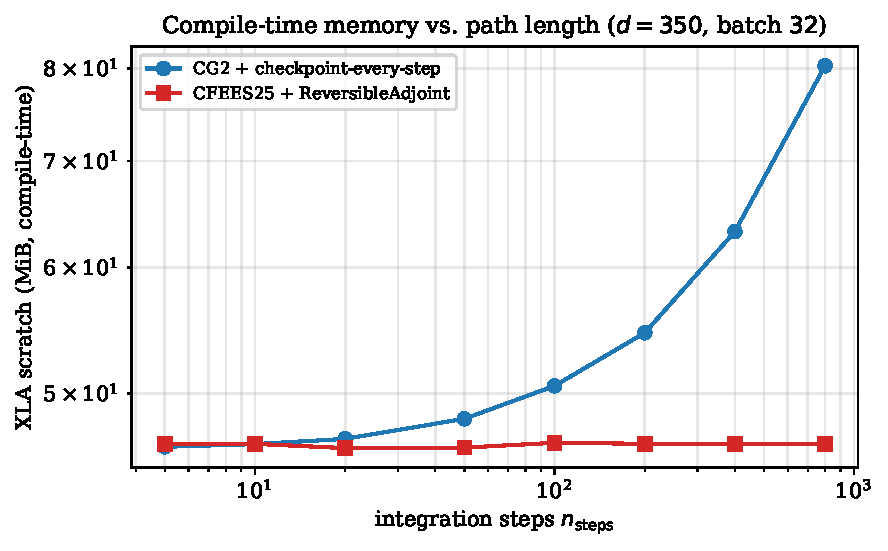
\includegraphics[width=0.85\linewidth]{fig_scaling.pdf}
\caption{XLA compile-time scratch for one forward+backward
training step on the torus neural SDE at $d=350$, batch $32$.
Each point is a fresh Python subprocess reading
\texttt{temp\_size\_in\_bytes} off the compiled executable.
\cfees{} under \texttt{ReversibleAdjoint} (red) is flat at
$46.5\,\mathrm{MiB}$ across $5 \leq n_{\mathrm{steps}} \leq 800$,
the $\mathcal{O}(1)$ behaviour predicted by reversibility.
\cgtwo{} (blue) and \cgfour{} (green) under
\texttt{RecursiveCheckpointAdjoint(checkpoints$=n_{\mathrm{steps}}$)}
both grow linearly at a slope of $\sim\!0.043\,\mathrm{MiB}$ per
step, matching $d \cdot B \cdot 4\,\mathrm{B} = 0.044\,\mathrm{MiB}$
for float$32$ activations to within $2\%$. The two curves share the
same slope: solver order does not change the memory complexity
under checkpointing, because each snapshot stores only the ODE
state $y$, not the stage values. \cgfour{} sits
$\sim\!3\,\mathrm{MiB}$ above \cgtwo{} as a constant offset from
its larger stage tableau.}
\label{fig:scaling}
\end{figure}

Table~\ref{tab:scaling} gives the exact numbers. The ratio
$\mathrm{CG2{:}checkpoint\_full} / \mathrm{CFEES25{:}reversible}$
reaches $1.72\times$ at $n_{\mathrm{steps}} = 800$ and extrapolates
to $10.2\times$ at $n_{\mathrm{steps}} = 10{,}000$ using the
measured linear slope; \cgfour{} is essentially parallel, a couple
of percent higher.

\begin{table}[hbt]
\centering
\small
\caption{XLA compile-time scratch (MiB) for one forward+backward
training step at $d = 350$, batch $32$, hidden $128$,
$\mathrm{d}t = 0.05$. \cfees{} uses \texttt{ReversibleAdjoint};
\cgtwo{} and \cgfour{} use
\texttt{RecursiveCheckpointAdjoint(checkpoints=$n_{\mathrm{steps}}$)}.}
\label{tab:scaling}
\begin{tabular}{r rrr r}
\toprule
$n_{\mathrm{steps}}$ & \cfees{} & \cgtwo{} & \cgfour{} & \cgtwo{}$/$\cfees{} \\
\midrule
  $5$ & $\mathbf{46.3}$ & $46.7$ & $49.0$ & $1.01\times$ \\
 $10$ & $\mathbf{46.5}$ & $46.5$ & $49.2$ & $1.00\times$ \\
 $20$ & $\mathbf{46.6}$ & $46.9$ & $49.2$ & $1.01\times$ \\
 $50$ & $\mathbf{46.5}$ & $48.2$ & $50.1$ & $1.04\times$ \\
$100$ & $\mathbf{46.5}$ & $50.5$ & $52.3$ & $1.09\times$ \\
$200$ & $\mathbf{46.7}$ & $54.6$ & $56.5$ & $1.17\times$ \\
$400$ & $\mathbf{46.3}$ & $63.2$ & $64.9$ & $1.37\times$ \\
$800$ & $\mathbf{46.8}$ & $80.4$ & $82.8$ & $1.72\times$ \\
\bottomrule
\end{tabular}
\end{table}

\paragraph{Wall clock.}
The same sweep records mean forward+backward wall clock over five
timed repetitions after one warmup. At $n_{\mathrm{steps}} = 800$
with $d=350$, \cfees{}$+$\texttt{ReversibleAdjoint} runs in
$5.02\,\mathrm{s}$ versus $3.09\,\mathrm{s}$ for
\cgtwo{}$+$checkpoint-every-step and $3.37\,\mathrm{s}$ for
\cgfour{}: the reversible scheme pays a $1.49$--$1.62\times$
wall-clock penalty in exchange for constant memory. This is the
expected time--memory trade-off of reversibility: one extra forward
per backward is amortised across the integration loop. At small
$n_{\mathrm{steps}}$ the absolute overhead of the reversible
backward is dominated by the constant Python and JAX dispatch cost
that applies to every solver step, and the wall-clock gap closes.

\section{Conclusion}

The flat $d$-torus is a clean Lie-group test bench for the
asymptotic memory claim of the \cfees{} family.
Figure~\ref{fig:scaling} makes the theoretical statement
$\mathcal{O}(1)$ vs $\mathcal{O}(n_{\mathrm{steps}})$ concretely
visible at $d = 350$: the reversible adjoint's compile-time
scratch is flat at $46.5\,\mathrm{MiB}$ across two orders of
magnitude of path length, while storing one activation snapshot
per step grows linearly at a rate dictated by the state size
times batch size times float precision --- independent of solver
order, as the \cgtwo{} and \cgfour{} curves confirm. The ratio is
modest at $n_{\mathrm{steps}}$ in the dozens but reaches
$1.72\times$ at $n_{\mathrm{steps}} = 800$ and diverges in the
limit. Combined with the $\mathrm{SPD}(n)$ companion experiment,
which exercises the noncommutative machinery and reports the
$5.6$--$23\times$ figures characteristic of the large ambient
spaces typical of that setting, this gives a complete picture of
where the reversible \cfees{} adjoint helps and how much.

\paragraph{Implementation.}
GRU encoder: hidden $128$, output $c \in \Reals^{64}$. Drift and
diffusion MLPs: depth $3$ and $2$, width $128$, $\mathrm{silu}$;
diffusion closes with $\mathrm{softplus}$ at bias $-2.0$ and scale
$\sigma_W = 0.1$. Representative chains come from the BGSU
non-redundant RNA list at $3.0\,$\AA{} resolution, parsed from
mmCIF via \texttt{biotite}; we keep contiguous runs of $\geq 30$
residues with all seven dihedrals defined and split by deterministic
chain hash. Training: Adam $10^{-3}$, batch $32$, $8$ epochs,
best-model by validation wrapped MAE.

\end{document}
